\Chapter{Tervezés}

Itt kezdődik a dolgozat lényegi része, úgy értve, hogy a saját munka bemutatása.
Jellemzően ebben szerepelni szoktak blokkdiagramok, a program struktúrájával foglalkozó leírások.
Ehhez célszerű UML ábrákat (például osztály- és szekvenciadiagramokat) használni.

Amennyiben a dolgozat inkább kutatás jellegű, úgy itt lehet konkretizálni a kutatási módszertant, a kutatás tervezett lépéseit, az indoklást, hogy mit, miért és miért pont úgy érdemes csinálni, ahogyan az a későbbiekben majd részletezésre kerül.

Ebben a fejezetben az implementáció nem kell, hogy túl nagy szerepet kapjon.
Ez még csak a tervezési fázis.
(Nyilván ha olyan a téma, hogy magának az implementációnak a módjával foglalkozik, adott formális nyelvet mutat be, úgy a kódpéldákat már innen sem lehet kihagyni.)

\Section{Követelmények}
A probléma szimulációja 3 programból \ref{fig:3program} áll. Egy program az adatközpont, egy program a drónok szerepét veszi fel, a harmadik program vezéreli a szimulációt,
tehát igazából csak paraméterek alapján konfigurálja a másik 2 program működését. Az első két program mikroszervízes struktúrában használhatónak kell lennie, hogy a konkurrens működést megfelelően tudjuk tesztelni.\\
Az adatközpontot szimuláló program lesz a legbonyolultabb. Ennek a programnak tudnia kell hibamentesen, adatvesztés nélkül
feldolgozni és tárolnia az adatokat amiket a drónok küldenek, és vezérelni kell tudni a drónok indítását, logisztikai feladatait.

\begin{figure}[h]
    \centering
    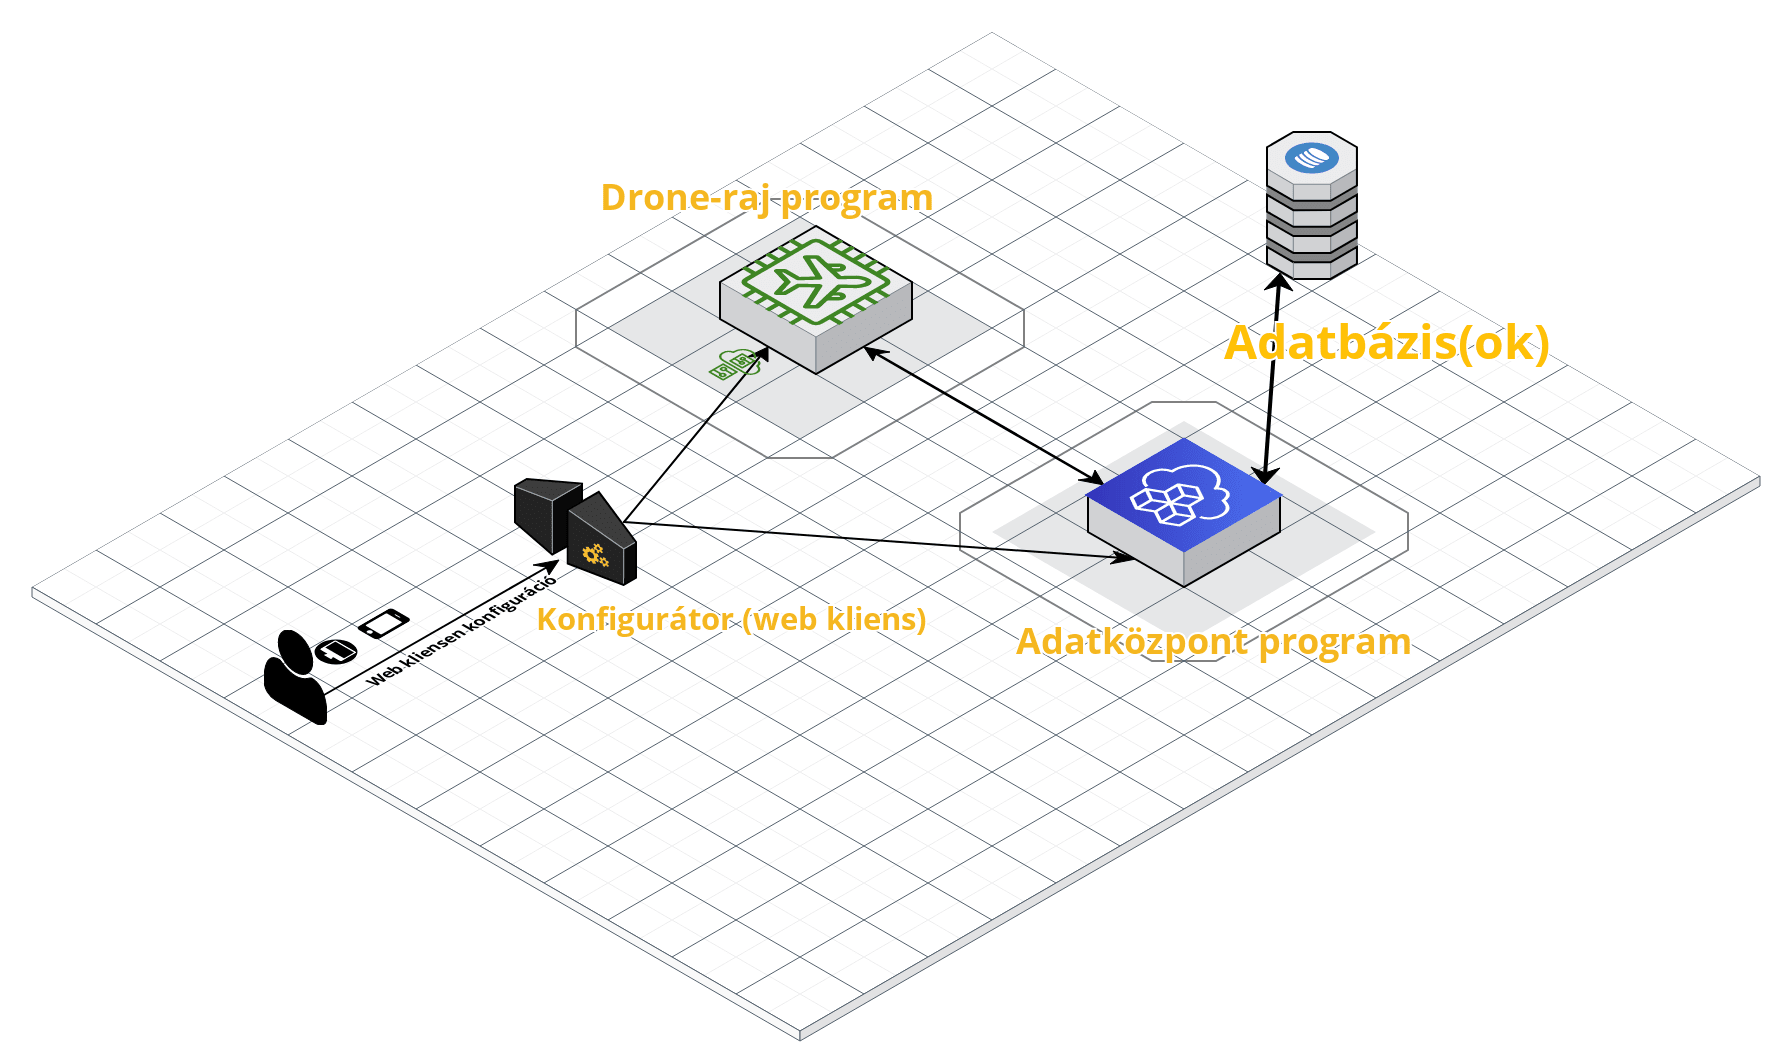
\includegraphics[scale=0.2]{images/szakdolgozat-3-program-abra.png}
    \caption{Hexagonal architecture driver and driven actors}
    \label{fig:3program}
\end{figure}


A szimulációban több féle protokolt és adattovábbításra képes formátumot hasonlítunk össze, így a programot úgy kell felépíteni,
hogy ki lehessen cserélni ezeket a végpontokat anélkül hogy a program üzleti logikájának működését befolyásolnánk. Az adatközpontok és drónok közötti kommunikációt és adatfeldolgozást összehasonlítjuk
egy HTTP 1.1 -en műkodő JSON adatformátumot használó REST API-n, egy HTTP 2 -n futó gRPC API-n és egy MQTT protokollt használó végponton is.

Az adatok adatbázisba mentése, adatbázisból olvasása közben több probléma merülhet fel, a rendszer konkurrens felépítéséből kiindulva.
Például amikor az épp szabad drónoknak adunk feladatot, lehet hogy 2 vagy több egyede az adatközpont programunknak kiolvassa azt az értéket hogy
a drón nem csinál semmit, az állapota szabad, adhat neki feladatot ha van szállítsra váró csomag. De, az üzleti logika futtatása közben az egyik egyed módosíthatta
az értéket arra hogy már repül, vagy épp csomagot vesz fel. Az ilyen Lost Update problémákkal szemben a program implementációjának ellenállónak kell lennie.

A adatközpont programnak elosztott rendszerként kell működnie, tehát terheléselosztás és megfelelő vezérlés szükséges.
\Section{Program struktúra}
\subsection{Architektúra, program felépítés}
Ahhoz hogy a programot a követelmányben megfogalmazott módon építsük fel, értem ezalatt azt hogy több protokollt és adatbázist hasonlítsunk össze egy olyan
program architektúrát, felépítést kell választani ami megendegi ezt.
Erre a problémára megoldásként a Hexagonal architektúrát \ref{fig:hexagonal-inward} és DDD tervezési alapelvet fogom alkalmazni.
\begin{figure}[h]
    \centering
    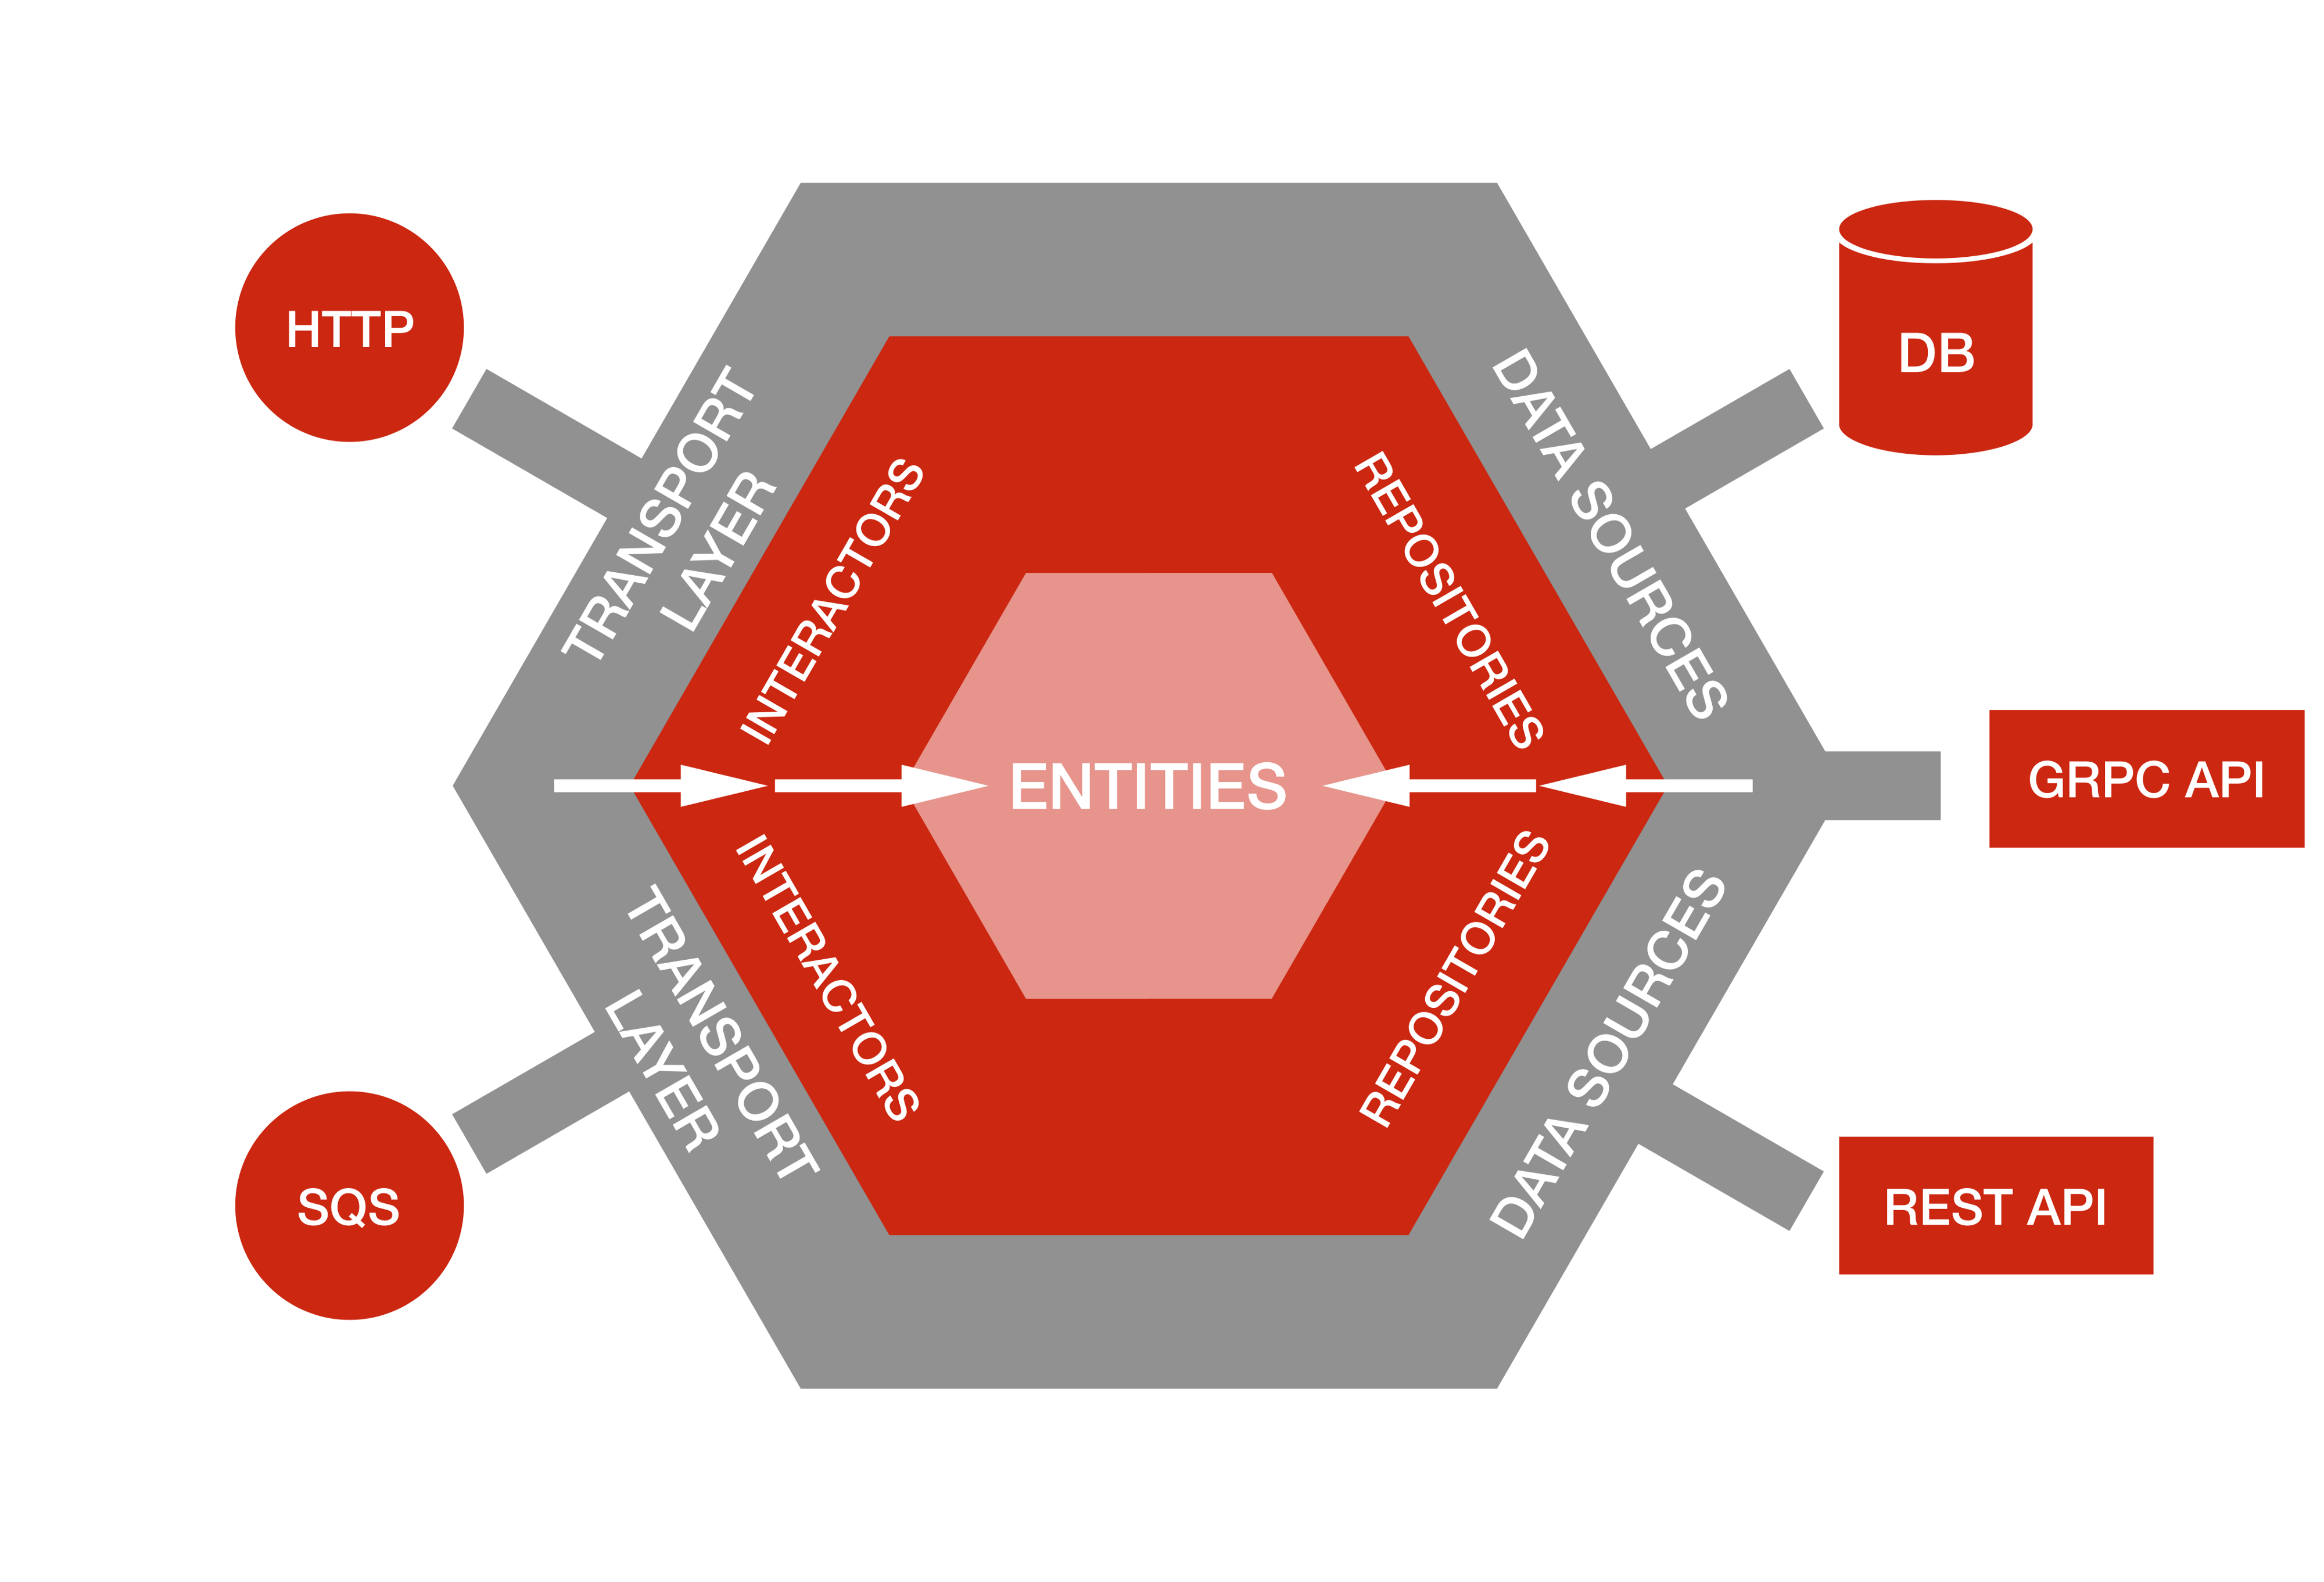
\includegraphics[scale=0.07]{images/hexa-inward.png}
    \caption{Hexagonal architecture inward pointing dependencies}
    \label{fig:hexagonal-inward}
\end{figure}
Így a program belülről kifelé rétegesen epül fel, interfaceket alkalmazva, úgy hogy a pontos implemetáció absztraktálva van, az csak az üzleti logikát ismerjük biztosan, minden ráépülő réteg implementációja cserélhető marad.
Minden réteg csak befelé mutat \ref{fig:hexagonal-inward}, így az üzleti logikánk megmaradhat, miközben az alkalmazás teljes infrastuktúráját kicserélhetnénk.
így a végpontok ha teljesítik az interface elvárásait, csak dependency injection-el kicseréljük a végpontot és minden ugyanúgy működik, ám teljesen más az implementáció.
Azt hogy több fajta input és output végpontot hogy  támogatja az alkalmazás a következő ábra \ref{fig:hexagonal-inward} tökéletesen bemutatja.
Az alkalmazást fel lehet osztani verérlő és vezérelt részre. Ez nagyon jól igazodik az üzleti logikához, egy inputra szinte mindig valamiféle vezérlést várunk el,
tehát hogyha az alkalmazásunkat használjuk, vezéreljük akkor az az adatok hatására valamit csináljon. Ezután az alkalmazásunk beszélhet más, külső forrásokkal, amiket az alkalmazás használ, azaz vezéreli őket.
Ilyen lehet egy adatbázis implementációja, vagy egy üzenet sor, amibe adatokat rakunk be, hogy valami más később kiolvassa.
Azért jó ez a felépítés, mert így például mindegy hogy a terminálból valamilyen konzolos applikáción keresztül hívjuk meg az alkalmazásunkat,
vagy egy webes felületről, esetleg mobil applikációból. A vezérelt egységeket is ki lehet cserélni, nem vagyunk röghöz kötve
mert egyszer így lett megírva az alkalmazésunk, csak a megfelelő réteget kicseréljük, feltéve hogy megírtuk hozzá az implementációnkat és az implementációnk
az intefészen keresztül teljesít minden feltételt. Így például könnyen átállhatunk r1elációs adatbázisról egy dokumentum alapúra, ha valami miatt úgy kívánjuk.
A Netflix is ezt az architektúrát használja \cite{netflix}, ugyanis a gyors növekedésük közben több skálázhatósággal összefüggő problémába ütköztek, amit úgy oldottak meg hogy
ebben az architektúrában\ref{fig:hexagonal-actor} szétosztották a feladatokat több, az adott kis feladatra megfelelő adatbázisra, mikroszervízre.
\begin{figure}[h]
    \centering
    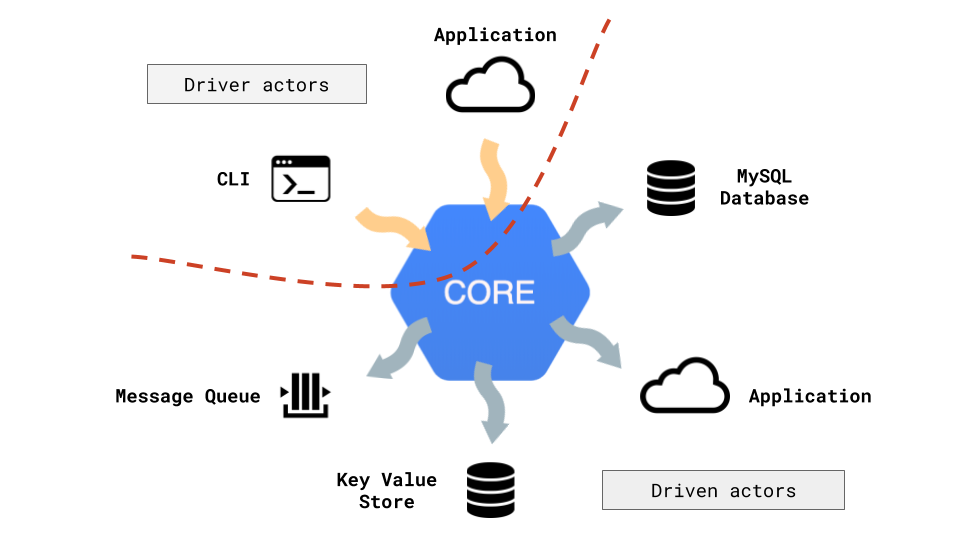
\includegraphics[scale=0.3]{images/hexa-actor.png}
    \caption{Hexagonal architecture driver and driven actors}
    \label{fig:hexagonal-actor}
\end{figure}
\\
A drón-raj program  olyan adatokat fog generálni, amelyet egy valós drónok generálnának és ezeket az adatokat tovább fogja küldeni az adatközpontnak.
%TODO: ide még írni és a program struktúráját jobban megmutatni, a konkrét jegyzék struktúra is akár, hogy mi tartozik infrastruktúrához, mi a program magja stb. Interfacek kapcsolata,
%TODO: Új section ami a program folyamatával foglalkozik, nem a struktúrával



%TODO: Még a struktúrához kell a Go-kit, azért lett ez választva mert nem framework, hanem egy library/ecosystem, így több szabadságot kap a program,
%hogy hogyan is lesz mikroszerviz. Go kit ben van service discovery,  beepitett Observability (Prometheus), többszintes logger, és A hexagonal architektúrát támogatja
%Pl más hasonló mikroszervizeket kezelő framework (pl. Micro) nem elég rugalmas, sok mindent nem enged meg, egy féleképpen lehet használni.



\section{Számítási problémák}

\paragraph{Cartesian szerinti}
\begin{gather}
    P_1(5,6,3) \\
    P_2(7,4,9) \\
    V = 10 \frac{m}{s}
\end{gather}


Kiszamitas:

\begin{gather}
    x = r * cos(\phi) * sin(\theta) \\
    y = r * sin(\phi) * sin(\theta) \\
    z = r * cos(\theta)
\end{gather}


X, Y, Z, r

\begin{gather}
    x = X_2 - X_1 = 7 - 5 = 2 \\
    y = Y_2 - Y_1 = 4 - 6 = -2 \\
    z = Z_2 - 7_1 = 9 - 3 = 6 \\
    r = \sqrt{2^2 + (-2)^2 + 6^2} = \sqrt{44}
\end{gather}

$
cos(\phi) sin(\phi) cos(\theta) sin(\theta)
$

\begin{gather}
    cos(\phi) = \frac{x}{\sqrt{x^2 + y^2}} \\
    sin(\phi) = \frac{y}{\sqrt{x^2 + y^2}} \\
    cos(\theta) = \frac{\sqrt(x^2 + y^2)}{\sqrt{x^2 + y^2 + z^2}} \\
    sin(\theta) = \frac{z}{\sqrt{x^2 + y^2 + z^2}}
\end{gather}

\newpage

További számítás segédvektorok kiszámítása:

\begin{gather}
    V_x = \frac{x}{\sqrt{x^2 + y^2 + z^2}} *V = \frac{2}{\sqrt{44}} * 10 = \frac{10\sqrt{11}}{11} = 3.0151\\
    V_y = \frac{y}{\sqrt{x^2 + y^2 + z^2}} *V = \frac{-2}{\sqrt{44}} * 10 = -\frac{10\sqrt{11}}{11} = -3.0151\\\\
    V_z = \frac{z}{\sqrt{x^2 + y^2 + z^2}} *V = \frac{6}{\sqrt{44}} * 10 = \frac{30\sqrt{11}}{11} = 9.0453\\
\end{gather}

Összesen eltelt idő:

\begin{gather}
    t = \frac{s}{v}
\end{gather}

\begin{gather}
    t_osszes = \frac{\sqrt{(x_2 - x_1)^2 + (y_2 - y_1)^2 + (z_2 - z_1)^2}}{v} = \frac{\sqrt{(7 - 5)^2 + (4 - 6)^2 + (9 - 3)^2}}{10} = \frac{\sqrt{44}}{10}{}
\end{gather}

t idő múlva egy adott pillanatban koordináták meghatározása:

\begin{gather}
    x = X_0 + V_x * t = X_0 + \frac{X}{\sqrt{x^2 + y^2 + z^2}} * t = 5 + \frac{2}{\sqrt{44}} * 10 * t \\
    Y = y_0 + V_y * t = y_0 + \frac{y}{\sqrt{x^2 + y^2 + z^2}} * t = 4 - \frac{2}{\sqrt{44}} * 10 * t \\
    z = z_0 + V_z * t = z_0 + \frac{z}{\sqrt{x^2 + y^2 + z^2}} * t = 6 + \frac{6}{\sqrt{44}} * 10 * t
\end{gather}

\paragraph{Az Ortodroma számítás, a föld alakját figyelembe véve}


Mivel gömbi geometria lényegesen eltér az euklideszi geometriától ezért a távolságszámításra használt matematikai képletek is eltérőek.
Az euklideszi geometriában a legrövidebb távolságot a két pontot összekötő egyenes,
a nem euklideszi geometriában a két pontot összekötő geodetikus vonal (gömb esetén főkör) mentén mérjük.

\begin{gather}
    d = acos(sin(\phi_1) * sin(\phi_2) * cos(\phi_1) * cos(\phi_2) * cos(\triangle \lambda)) * R
\end{gather}

\Section{Táblázatok}

Táblázatokhoz a \texttt{table} környezetet ajánlott használni.
Erre egy minta \aref{tab:minta}. táblázat.
A hivatkozáshoz az egyedi \texttt{label} értéke konvenció szerint \texttt{tab:} prefixszel kezdődik.

\begin{table}[h]
\centering
\caption{Minta táblázat. A táblázat felirata a táblázat felett kell legyen!}
\label{tab:minta}
\begin{tabular}{l|c|c|}
a & b & c \\
\hline
1 & 2 & 3 \\
4 & 5 & 6 \\
\hline
\end{tabular}
\end{table}

\Section{Ábrák}

Ábrákat a \texttt{figure} környezettel lehet használni.
A használatára egy példa \aref{fig:cimer}. ábrán látható.
Az \texttt{includegraphics} parancsba 
Az ábrák felirata az ábra alatt kell legyen.
Az ábrák hivatkozásához használt nevet konvenció szerint \texttt{fig:}-el célszerű kezdeni.

\begin{figure}[h]
\centering

\includegraphics[scale=0.3]{images/me_logo.png}
\caption{A Miskolci Egyetem címere.}
\label{fig:cimer}
\end{figure}

\Section{További környezetek}

A matematikai témájú dolgozatokban szükség lehet tételek és bizonyításaik megadására.
Ehhez szintén vannak készen elérhető környezetek.

\begin{definition}
Ez egy definíció
\end{definition}

\begin{lemma}
Ez egy lemma
\end{lemma}

\begin{theorem}
Ez egy tétel
\end{theorem}

\begin{proof}
Ez egy bizonyítás
\end{proof}

\begin{corollary}
Ez egy tétel
\end{corollary}

\begin{remark}
Ez egy megjegyzés
\end{remark}

\begin{example}
Ez egy példa
\end{example}

